Construct a $T^{2}$-chart using the data on $x_{1} = \text{legal appearances overtime hours}$,
$x_{2} = \text{extraordinary event overtime hours}$, and $x_{3} = \text{holdover overtime hours}$ from
Table 5.8. Compare this chart with the chart in Figure 5.8 of Example 5.10. Does plotting
$T^{2}$ with an additional characteristic change your conclusion about process stability?
Explain.

\begin{figure}[H]
    \centering
    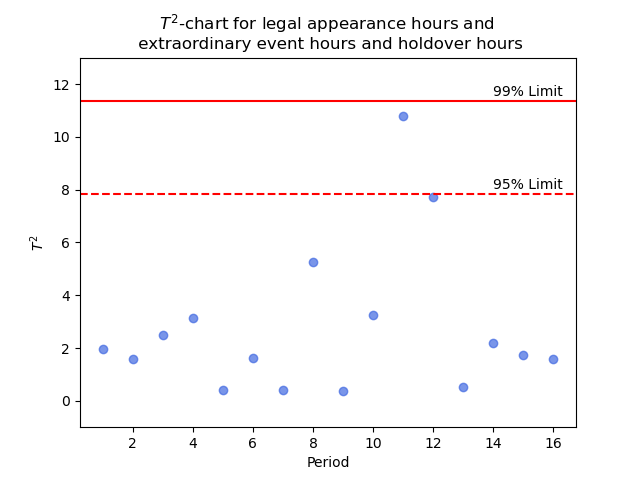
\includegraphics[scale=0.65]{./python/chapter-5/Question-5-26-T2.png}
\end{figure}

Including holdover overtime alters the chart seen in Figure 5.8. In the $T^{2}$ plot above we identify observation 11 as being outside the 95\% limit, but not outside the 99\% limit. In Figure 5.8 observation 11 is outside the 99\% limit. We can also see that observation 12 is almost outsie the 95\% limit, which in Figure 5.8, I'm assuming it's outside the 95\% limit. In figure 5.8, the upper control limit for $\alpha=0.01$ was $\chi_{p=2}^{2}(0.01) = 9.21$, and here $\chi_{p=3}^{2}(0.01) = 11.34$. Throwing another variable into the mix caused the upper control limits to become higher, and the $T^{2}$ values increased some, but not that much, so our data looks more stable than in Figure 5.8, even though the pattern in the data is roughly similar.
